\documentclass{article}

\usepackage{amsmath, amsthm, amssymb, amsfonts}
\usepackage{thmtools}
\usepackage{graphicx}
\usepackage{setspace}
\usepackage{geometry}
\usepackage{float}
\usepackage{hyperref}
\usepackage[utf8]{inputenc}
\usepackage[english]{babel}
\usepackage{framed}
\usepackage[dvipsnames]{xcolor}
\usepackage[most]{tcolorbox}
\usepackage{minted}
\usepackage{enumitem}
\usepackage{booktabs}
\usepackage{multirow}

\usepackage{indentfirst}

\usepackage[export]{adjustbox} % Align images

\colorlet{LightGray}{White!90!Periwinkle}
\colorlet{LightOrange}{Orange!15}
\colorlet{LightGreen}{Green!15}

\newcommand{\HRule}[1]{\rule{\linewidth}{#1}}

\newtcbtheorem[auto counter,number within=section]{code}{Código}{
  colback=LightOrange!20,
  colframe=LightOrange,
  colbacktitle=LightOrange,
  fonttitle=\bfseries\color{black},
  boxed title style={size=small,colframe=LightOrange},
}{code}

\setstretch{1.2}
\geometry{
  textheight=22.5cm,
  textwidth=13.75cm,
  top=2.5cm,
  headheight=12pt,
  headsep=25pt,
  footskip=30pt
}

% ------------------------------------------------------------------------------

\begin{document}

% ------------------------------------------------------------------------------
% Cover Page and ToC
% ------------------------------------------------------------------------------
\begin{center}
  \begin{figure}
    \includegraphics[scale = 0.3, left]{img/IST_A.eps} % IST logo
    \end{figure}
  \LARGE{ \normalsize \textsc{} \\
  [2.0cm] 
  \LARGE{ \LARGE \textsc{Machine Learning}} \\
  [1cm]
  \LARGE{ \LARGE \textsc{LEIC IST-UL}} \\
  [1cm]
  \HRule{1.5pt} \\
  [0.4cm]
  \LARGE \textbf{\uppercase{Relatório - Homework 1}}
  \HRule{1.5pt}
  \\ [2.5cm]
  }
\end{center}

\begin{flushleft}
  \textbf{\LARGE Grupo 10:}
\end{flushleft}

\begin{center}
  \begin{minipage}{0.7\textwidth}
      \begin{flushleft}
        \large Gabriel Ferreira \\
        \large  Irell Zane
      \end{flushleft}
  \end{minipage}%
  \begin{minipage}{0.3\textwidth}
      \begin{flushright}
        \large 107030\\
        \large 107161
      \end{flushright}
  \end{minipage}
\end{center}

\begin{center}
  \vspace{4cm}
  \date \large \bf  2024/2025 -- 1st Semester, P1
\end{center}

\setcounter{page}{0}
\thispagestyle{empty}
\renewcommand{\thesection}{\Roman{section}}

\newpage

% ------------------------------------------------------------------------------
% Content
% ------------------------------------------------------------------------------



\large{\textbf{Part I}: Pen and paper}\normalsize




\begin{enumerate}[leftmargin=\labelsep]
\item Completion of the decision tree.

\vspace{3pt}

\begin{minipage}{0.4\textwidth}
  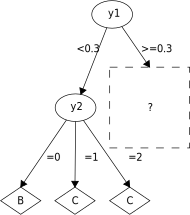
\includegraphics[scale = 0.3, left]{img/decision_tree_1.pdf}
\end{minipage}
\hspace{0.05\textwidth}
\begin{minipage}{0.6\textwidth}
  The node we must decide what to do with is to the right
  of the root, with the dataset $D | (y1 >= 0.3)$.
  \begin{table}[H]
    \centering
    \begin{tabular}{@{}ccccc}
      $D | (y1 >= 0.3)$ & $y_2$ & $y_3$ & $y_4$ & $y_{out}$ \\ \midrule
      $x_6$  & 0 & 1 & 0 & B \\
      $x_7$  & 0 & 1 & 1 & A \\
      $x_8$  & 1 & 0 & 0 & A \\
      $x_9$  & 0 & 1 & 1 & C \\
      $x_{10}$ & 0 & 1 & 1 & C \\
      $x_{11}$ & 1 & 0 & 0 & A \\
      $x_{12}$ & 1 & 2 & 0 & B \\
    \end{tabular}
  \end{table}

  Since there are distinct $y_{out}$ values, and more 
  than 4 observations. This this node should be split.
\end{minipage}
\vspace{3pt}
 
To decide the next variable to use, we must calculate 
the Information Gain of each variable using Shannon 
entropy for the dataset.
Considering $X_i$ is a subset of $D | (y1 >= 0.3)$:


\begin{equation*}
  H(y_{out}|X_i) = -p(A|X_i)log_2(p(A|X_i))-p(B|X_i)log_2(p(B|X_i))-p(C|X_i)log_2(p(C|X_i))
\end{equation*}

\begin{equation*}
  H(y_{out}|y_j) = \sum^{i}p(X_i) H(y_{out}|X_i)
\end{equation*}

\begin{equation*}
  IG(y_j) = H(y_{out}) - H(y_{out}|y_j)
\end{equation*}

Entropy of the $D | (y1 >= 0.3)$ set:

\begin{equation*}
  H(y_{out}) = -\frac{3}{7}log_2(\frac{3}{7})-\frac{2}{7}log_2(\frac{2}{7})-\frac{2}{7}log_2(\frac{2}{7}) = 1.57
\end{equation*}

\begin{table}[H]
  \begin{tabular}{cc|ccccc|cc}
  $j$ & $X_i$                    & $p(X_i)$        & $p(A | X_i)$   & $p(B | X_i)$   & $p(C | X_i)$   & $H(y_{out}|X_i)$ & $H(y_{out}|y_j)$ & $IG(y_{out}|y_j)$ \\ \midrule
  \multirow{2}{*}{2} & $y_2=0$ & $\frac{4}{7}$ & $\frac{1}{4}$ & $\frac{1}{4}$ & $\frac{2}{4}$ & 1.5  & \multirow{2}{*}{1.25} & \multirow{2}{*}{0.31} \\
   &                   $y_2=1$ & $\frac{3}{7}$ & $\frac{2}{3}$ & $\frac{1}{3}$ & $\frac{0}{3}$ & 0.92 &  &  \\ \midrule
  \multirow{3}{*}{3} & $y_3=0$ & $\frac{2}{7}$ & $\frac{2}{2}$ & $\frac{0}{2}$ & $\frac{0}{2}$ & 0    & \multirow{3}{*}{\textbf{0.86}} & \multirow{3}{*}{\textbf{0.70}} \\
   &                   $y_3=1$ & $\frac{4}{7}$ & $\frac{1}{4}$ & $\frac{1}{4}$ & $\frac{2}{4}$ & 1.5  &  &  \\
   &                   $y_3=2$ & $\frac{1}{7}$ & $\frac{0}{1}$ & $\frac{1}{1}$ & $\frac{0}{1}$ & 0    &  &  \\ \midrule
  \multirow{2}{*}{4} & $y_4=0$ & $\frac{4}{7}$ & $\frac{2}{4}$ & $\frac{2}{4}$ & $\frac{0}{4}$ & 1    & \multirow{2}{*}{0.96} & \multirow{2}{*}{0.60} \\
   &                   $y_2=4$ & $\frac{3}{7}$ & $\frac{1}{3}$ & $\frac{0}{3}$ & $\frac{2}{3}$ & 0.92 &  &  \\ \bottomrule
  \end{tabular}
\end{table}

As seen in the table above, $y_3$ is the variable with the 
most information gain, it is the one that should be chosen 
to split the node.
Dividing the node's dataset into 3 subsets:

\vspace{-3pt}

\begin{minipage}[t]{0.3\textwidth}
  \begin{table}[H]
    \centering
    \begin{tabular}{@{}cccc}
      $y_3 = 0$ & $y_2$ & $y_4$ & $y_{out}$ \\ \midrule
      $x_8$    & 1 & 0 & A \\
      $x_{11}$ & 1 & 0 & A \\
    \end{tabular}
  \end{table}
\end{minipage}
\begin{minipage}[t]{0.3\textwidth}
  \begin{table}[H]
    \centering
    \begin{tabular}{@{}cccc}
      $y_3 = 1$ & $y_2$ & $y_4$ & $y_{out}$ \\ \midrule
      $x_6$    & 0 & 0 & B \\
      $x_7$    & 0 & 1 & A \\
      $x_9$    & 0 & 1 & C \\
      $x_{10}$ & 0 & 1 & C \\
    \end{tabular}
  \end{table}
\end{minipage}
\begin{minipage}[t]{0.3\textwidth}
  \begin{table}[H]
    \centering
    \begin{tabular}{@{}cccc}
      $y_3 = 2$ & $y_2$ & $y_4$ & $y_{out}$ \\ \midrule
      $x_{12}$ & 1 & 0 & B \\
    \end{tabular}
  \end{table}
\end{minipage}

\vspace{5pt}
\fbox{
\begin{minipage}{0.50\textwidth}
  \textbf{Solution} \\
  \includegraphics[scale = 0.25, left]{img/decision_tree_3.pdf}
\end{minipage}
\hspace{0.01\textwidth}
}
\hspace{0.02\textwidth}
\begin{minipage}{0.47\textwidth}
  The subset where $y_3=1$ is another candidate for splitting,
  since it has at least 4 observations.
  The choice of variable is trivially $y_4$, since $y_2$ has no 
  information gain, and every other variable has been split.

  Now every subset has less than 4 observations.
  $y_4=1$ is C because it's the most common, and 
  $y_4=2$ is A, because, having no observations, ascending
  alphabetic order is prioritized.
\end{minipage}

\vfill

\item Draw the confusion Matrix.

\begin{minipage}{0.50\textwidth}
  \begin{table}[H]
    \centering
    \begin{tabular}{ccc}
      D & Target  & Predicted \\ \midrule
      $x_1$     & C & C \\
      $x_2$     & B & B \\
      $x_3$     & C & C \\
      $x_4$     & B & B \\
      $x_5$     & C & C \\
      $x_6$     & B & B \\
      $x_7$     & A & C \\
      $x_8$     & A & A \\
      $x_9$     & C & C \\
      $x_{10}$  & C & C \\
      $x_{11}$  & A & A \\
      $x_{12}$  & B & B \\
    \end{tabular}
  \end{table}
\end{minipage}
\fbox{
\begin{minipage}{0.30\textwidth}
  \centering
  \textbf{Solution} \\
  \begin{table}[H]
    \centering
    \begin{tabular}{@{}ccccc}
      & \multicolumn{4}{c}{\small{Target}} \\
      &   & A & B & C \\ \cmidrule(l){2-5} 
      \multirow{3}{*}{\rotatebox{90}{\small{Predicted}}}
      & A & 2 & 0 & 0 \\
      & B & 0 & 4 & 0 \\
      & C & 1 & 0 & 5 \\
    \end{tabular}
  \end{table}
\end{minipage}
}

\vfill

\newpage

\item Identify which class has the lowest training F1 score.

For this we will calculate Recall and Precision for each class.

\large{
\begin{minipage}[]{0.3\textwidth}
  \begin{equation*}
    \text{Recall} = \frac{TP}{TP + FN}
  \end{equation*}
\end{minipage}
\begin{minipage}[]{0.3\textwidth}
  \begin{equation*}
    \text{Precision} = \frac{TP}{TP + FP}
  \end{equation*}
\end{minipage}
\begin{minipage}[]{0.3\textwidth}
  \begin{equation*}
    \text{F1 Score} = \frac{2}{\frac{1}{P}+\frac{1}{R}}
  \end{equation*}
\end{minipage}
}

\vspace{3pt}

\fbox{
\begin{minipage}{\textwidth}
  \centering
  \vspace{3pt}
  \textbf{Solution} \\
  \begin{table}[H]
    \centering
    \large
    \begin{tabular}{ccccccr}
        & TP & FN & FP & Precision     & Recall & F1 Measure \\ \midrule
      A & 2  & 0  & 1  & $\frac{2}{2}$ & $\frac{2}{2+1}$ & $\frac{2}{1 + \frac{3}{2}} = \textbf{0.80} $ \\
      B & 4 & 0 & 0    & $\frac{4}{4}$ & $\frac{4}{4}$ & $\frac{2}{1 + 1} = 1.00 $ \\
      C & 5 & 1 & 0    & $\frac{5}{5+1}$ & $\frac{5}{5}$ & $\frac{2}{\frac{6}{5} + 1} \approx 0.91$ \\
    \end{tabular}
  \end{table}
  \textbf{Class A has the lowest F1 Score.}
  \vspace{3pt}
\end{minipage}
}
\vspace{10pt}



\item Draw the class-conditional relative histograms of y1.

\includegraphics[scale = 0.45, center]{img/histogram1_4.pdf}

If we split the root between each of these five bins, 
considering the class majority as a leaf node
(and the first alphabetically when tied), 
we wind up with the following 5-ary root split:

\vfill

\fbox{
\centering
\begin{minipage}{\textwidth}
  \centering
  \textbf{Solution} \\
  \begin{table}[H]
    \centering
    \begin{tabular}{ccccc}
      $[0; 0.20[$ & $[0.20; 0.40[$ & $[0.40; 0.60[$ & $[0.60; 0.80[$ & $[0.80; 1]$ \\ \midrule
      C & B & C & A & A 
    \end{tabular}
  \end{table}
\end{minipage}
}
\end{enumerate}

\vfill

\newpage

\large{\textbf{Part II}: Programming}\normalsize

\begin{enumerate}[leftmargin=\labelsep]
\item Glucose is the feature with the most discriminative power (\textbf{213.16}).
Blood Pressure is the feature with the least discriminative power (\textbf{3.26}).
\begin{center}
    \begin{minipage}[t]{0.45\textwidth}
        \centering
        \includegraphics[width=\textwidth]{img/best_disc_feature.png} 
    \end{minipage}
    \hfill
    \begin{minipage}[t]{0.45\textwidth}
        \centering
        \includegraphics[width=\textwidth]{img/worst_dict_feature.png} 
    \end{minipage}
\end{center}

\vfill

\item Plot of the results:
\begin{center}
    \includegraphics[width=0.5\textwidth]{img/tree_acc_vs_split.png} 
\end{center}

\vfill

\item With a very small minimum samples split number, the decision
tree is prone to overfitting to the training data, which is reflected
in a less adequate testing accuracy.

The training accuracy notably decreases as the minimum samples
split increases, and so does the testing accuracy after 50 minimum
samples --- because not having a huge pool of training data,
the process gets detrimentally more limited in the number of splits
it can make (underfitting).

To achieve the best generalization capacity, the minimum samples
split should be set to somewhere inbetween, where neither overfitting
nor underfitting is an issue. In this run the optimal peak is at 50 
minimum samples, where a testing accuracy of 76\% is achieved.

\vfill
\newpage

\item Decision Tree Plot:
    \begin{center}
        \includegraphics[width=0.9\textwidth]{img/tree_plot.png} 
    \end{center}

    \textbf{Glucose level is the primary factor}:
    \begin{itemize}
        \item If Glucose $\leq 127.5$: 19.4\% chance of diabetes
        \item If Glucose $> 127.5$: 61.6\% chance of diabetes
    \end{itemize}
    This shows that higher glucose levels are strongly associated with diabetes.

    \textbf{Age is a secondary factor for lower glucose levels}:
    \begin{itemize}
        \item If Glucose $\leq 127.5$ and Age $\leq 28.5$: 8.5\% chance of diabetes
        \item If Glucose $\leq 127.5$ and Age $> 28.5$: 33.2\% chance of diabetes
    \end{itemize}
    For people with lower glucose levels, being older increases the chance of diabetes.

    \textbf{BMI is important across different glucose and age ranges}:
    \begin{enumerate}[label=\alph*.]
        \item \textbf{For younger people with lower glucose}:
        \begin{itemize}
            \item If Glucose $\leq 127.5$, Age $\leq 28.5$, and BMI $\leq 45.4$: 7.5\% chance of diabetes
            \item If Glucose $\leq 127.5$, Age $\leq 28.5$, and BMI $> 45.4$: 75\% chance of diabetes
        \end{itemize}

        \item \textbf{For older people with lower glucose}:
        \begin{itemize}
            \item If Glucose $\leq 127.5$, Age $> 28.5$, and BMI $\leq 26.35$: 4.9\% chance of diabetes
            \item If Glucose $\leq 127.5$, Age $> 28.5$, and BMI $> 26.35$: 39.9\% chance of diabetes
        \end{itemize}

        \item \textbf{For people with higher glucose}:
        \begin{itemize}
            \item If Glucose $> 127.5$ and BMI $\leq 29.95$: 31.6\% chance of diabetes
            \item If Glucose $> 127.5$ and BMI $> 29.95$: 72.5\% chance of diabetes
        \end{itemize}
    \end{enumerate}
    Higher BMI is associated with a higher chance of diabetes.

    \textbf{For people with higher glucose and BMI, higher glucose levels further indicate the chance of diabetes}:
    \begin{itemize}
        \item If Glucose $> 127.5$, BMI $> 29.95$, and Glucose $\leq 157.5$: 60.9\% chance of diabetes
        \item If Glucose $> 127.5$, BMI $> 29.95$, and Glucose $> 157.5$: 87.0\% chance of diabetes
    \end{itemize}


\end{enumerate}

% ----------------------------------------------------------------------
% Cover
% ----------------------------------------------------------------------

\end{document}
